\documentclass[conference]{IEEEtran}
\IEEEoverridecommandlockouts
% The preceding line is only needed to identify funding in the first footnote. 
%If that is unneeded, please comment it out.

\usepackage{CCE}

\usepackage{cite}
\usepackage{amsmath,amssymb,amsfonts}
\usepackage{algorithmic}
\usepackage{graphicx}
\usepackage{textcomp}
\usepackage{xcolor}
\usepackage{float}
%\usepackage{hyperref}
\usepackage{adjustbox}
\usepackage{listings}

\definecolor{codegreen}{rgb}{0,0.6,0}
\definecolor{codegray}{rgb}{0.5,0.5,0.5}
\definecolor{codepurple}{rgb}{0.58,0,0.82}
\definecolor{backcolour}{rgb}{0.95,0.95,0.92}

\lstdefinestyle{mystyle}{
    backgroundcolor=\color{backcolour},
    commentstyle=\color{codegreen},
    keywordstyle=\color{magenta},
    numberstyle=\tiny\color{codegray},
    stringstyle=\color{codepurple},
    basicstyle=\ttfamily\footnotesize,
    breakatwhitespace=false,
    breaklines=true,
    captionpos=b,
    keepspaces=true,
    numbers=left,
    numbersep=5pt,
    showspaces=false,
    showstringspaces=false,
    showtabs=false,
    tabsize=2
}

\lstset{style=mystyle}

\def\BibTeX{{\rm B\kern-.05em{\sc i\kern-.025em b}\kern-.08em
    T\kern-.1667em\lower.7ex\hbox{E}\kern-.125emX}}
\begin{document}

\title{Characterization of Objects in Indoor Spaces of Human Occupation Using Knowledge Graphs\\ %*
% {\footnotesize \textsuperscript{*}Note: Sub-titles are not captured in Xplore and
% should not be used}
% \thanks{Identify applicable funding agency here. If none, delete this.}
}


\author
{
\IEEEauthorblockN{Rodrigo Francisco}
\IEEEauthorblockA{Engineering Faculty\\
National Autonomous University of Mexico\\
Mexico City, Mexico\\
% \href{mailto: holmesrodrigo@comunidad.unam.mx}{holmesrodrigo@comunidad.unam.mx}
holmesrodrigo@comunidad.unam.mx
}
\and
\IEEEauthorblockN{Guillermo Molero-Castillo}
\IEEEauthorblockA{Engineering Faculty\\
National Autonomous University of Mexico\\
Mexico City, Mexico\\
% \href{mailto: gmoleroca@fi-b.unam.mx}{gmoleroca@fi-b.unam.mx}
gmoleroca@fi-b.unam.mx
}
}


\maketitle

\begin{abstract}
In this paper, we propose a knowledge graph to describe the object semantic 
relationships that there are in an indoor space, such as a bedroom. To do so, 
we base our work on the representation model Object1--Predicate--Object2. In 
the predicate, we consider spatial relationships such as above, below, under, 
on top, next to, in, has, in front, and behind. To fulfill our purpose, it was 
used the Grakn NoSQL database, which allows defining a knowledge graph schema of
type entity-relation. The obtained knowledge graph needs a previously identified 
object in order to start looking for the correct relationships. That object is 
considered as input to the algorithm. The information on the semantic 
relationship has demonstrated its effectiveness in characterizing objects using 
Grakn, through which it was possible to characterize objects and their 
relationships based on the principles of knowledge representation.
\end{abstract}

\begin{IEEEkeywords}
    Knowledge Graphs, Grakn, indoor spaces, objects, semantic relationships.
\end{IEEEkeywords}
\section{Introduction}
Within the past ten years, object recognition
has gained importance due to the significant development of 
hardware (CPUs and GPUs with higher performance and speed) and thanks to the 
constant progress of computer science (increasingly sophisticated machine 
learning, and deep learning algorithms). Object detection involves two main 
tasks: i) image classification and ii) object localization.
% En los últimos 10 años, el reconocimiento de objetos, una rama de la 
% inteligencia artificial ha cobrado gran importancia debido al increíble 
% desarrollo del hardware (CPUs y GPUs con un mayor rendimiento y velocidad) y 
% gracias al constante progreso de la ciencia computacional (algoritmos de 
% machine learning y deep learning cada vez más sofisticados). La detección de 
% objetos involucra dos tareas principales: 
% i) la clasificación de imágenes y 
% ii) la  localización de objetos.

Image classification is intended to predict what kind of objects are in 
an image and object localization is about locating the object 
with a bounding box. In general, object recognition uses artificial 
neural networks, which despite being a powerful tool, they have the disadvantage 
of becoming slow through the large number (millions) of node networks 
communicating with each other. Hence, it is been necessary to propose different 
approaches to reduce processing time, thats why we address knowledge graphs.
% En primer lugar, la clasificación de imágenes tiene como objetivo predecir 
% la clase de objetos que hay en una imagen. Por otra parte, la localización de 
% objetos se refiere a indicar la localización de los objetos mediante una caja 
% o cuadro delimitador, generalmente conocido como \textit{bounding box}. 
% En general, para el reconocimiento de objetos se trabaja generalmente con 
% redes neuronales artificiales, las cuales, a pesar de ser una poderosa 
% herramienta, tienen la desventaja de llegar a ser lentas debido a la gran 
% cantidad (millones) de redes de nodos comunicadas entre sí. Por lo cual, ha 
% sido necesario plantear posibles soluciones para disminuir el tiempo de 
% procesamiento, como los grafos de conocimiento.

A knowledge graph is a set of organized information, where each vertex 
represents the specific data which can be accessed through a specific edge. 
% % Un grafo de conocimiento (KG) es un conjunto de información organizada, 
% donde cada vértice representa datos a los que se podrán acceder a través de 
% una arista. De la misma manera, \cite{Barnard} explica que un grafo de 
% conocimiento es una enciclopedia que las máquinas puede leer. Por lo que, 
% básicamente se trata de un conocimiento organizado de tal manera que una 
% máquina puede entender y extraer la información de forma fácil.
On the other hand, \cite{Saorin} points out that a knowledge graph connected 
with a database enriches and increases its
significance, for that reason entities and properties can be defined, thus those 
properties get classified and model  into our domain of knowledge. By having 
the domain to which it belongs, it allows another graph to connect it to another 
domain model.
% Por otro lado, \cite{Saorin} señala que un grafo de conocimiento está 
% integrado a una base de datos que al momento de unirse, el grafo se enriquece 
% e incrementa su significancia, lo cual permite que se definan entidades y 
% propiedades, las cuales se tipifican y clasifican para después modelarlas en 
% su dominio de conocimiento. Al tener el dominio al que pertenece, permite que 
% otro grafo pueda conectarlo a otro modelo de dominio.

The following example illustrates the previous idea: A system understands that 
a person being is an entity of soccer player type, and it is linked with soccer 
sport, which is played with a ball and where there are many competitions. 
In this way, a knowledge graph may have the following content related in a 
semantic way:
% El siguiente ejemplo ilustra la idea anterior: Un sistema entiende que una 
% entidad del tipo futbolista es un ser humano, y que está vinculado con el 
% deporte fútbol, que se juega con una pelota y donde hay una serie de 
% competiciones. Así, un grafo de conocimiento puede contener el siguiente 
% contenido relacionado de forma semántica:

\begin{itemize}
% \item Datos sobre un lugar, una persona o una empresa determinada.
\item Data of place, a person or a certain company.
% \item Imágenes.
\item Images.
% \item Extractos de texto.
\item Text excerpts.
% \item Datos con detalles secundarios.
\item Data with secondary details.
% \item Referencias a búsquedas similares.
\item References to similar searches.
\end{itemize}

This paper seeks to communicate the use of a knowledge graph as a tool to 
characterize the semantic relationships that exist between objects existing 
in a certain closed environment of human occupation, such as a room in a home, 
office, and other places of rest or work. To achieve this purpose, we use a 
basic model with three components : object1-predicate-object2. 
In predicate we use spatial relations such as: above, below, 
above, beside, in, has, in front and others.
% En este artículo se busca exponer el uso de un grafo de conocimiento como 
% herramienta para la caracterización de las relaciones semánticas que existen 
% entre los objetos existentes en un determinado ambiente cerrado de ocupación 
% humana, como una habitación de una vivienda, oficina y otros lugares de 
% descanso o trabajo. Para lograr este propósito se tomó como base el modelo 
% formado por tres componentes: object1-predicate-object2. Para el predicado 
% se consideró la relación de espacialidad como: arriba, abajo, encima, al lado, 
% en, tiene, en frente y otras.

The document is organized as follows, Section 2 presents the background of the 
degrees of knowledge, their applications are discussed and related works are 
presented. Section 3 describes the method established as a proposed solution. 
Section 4 presents the results obtained, based on an example of application in 
a room, and Section 5 summarizes some conclusions and future work.
% El documento está organizado de la siguiente manera, la Sección 2 presenta 
% los antecedentes de los grados de conocimiento, se discute sus aplicaciones y 
% se presentan los trabajos relacionados. La Sección 3 describe el método 
% establecido como propuesta de solución. La Sección 4 presenta los resultados 
% obtenidos, basado en un ejemplo de aplicación en una habitación, y la Sección 
% 5 resume algunas conclusiones y trabajo futuro.
\section{Background}

All recent efforts to work with object recognition successfully can be 
encompassed in two large model families. At first we have algorithms 
related to convolutional neural networks (CNN), and  in second place  the YOLO 
(You Only Look Once) approach.
% Todos los esfuerzos recientes para el reconocimiento de objetos de manera 
% satisfactoria se pueden englobar en dos grandes familias de modelos. En primer 
% lugar se tiene la utilización de algoritmos relacionados con redes neuronales 
% convolucionales (CNN), y en segundo lugar se tiene el enfoque YOLO (You Only 
% Look Once).

Models based on convolutional neural networks, as the name implies, use neural 
networks with an extra layer called the convolution layer, which has the 
characteristic of choosing or detecting patterns and making sense of them. 
Such pattern detection is what makes CNN useful for image analysis. CNN works 
through filters, which allow detecting patterns such as circles, edges, squares, 
lines, among others. The famous CNN-based models are: R-CNN, Fast R-CNN, and 
Faster R-CNN.
% Los modelos basados en redes neuronales convolucionales, como su nombre lo 
% indica, utilizan redes neuronales con una capa extra llamada capa de 
% convolución, la cual tiene la característica de escoger o detectar patrones 
% y darles sentido. Dicha detección de patrones es lo que hace que CNN sea útil 
% para el análisis de imágenes. Las CNN trabajan a través de filtros, los cuales 
% permiten detectar patrones como círculos, bordes, cuadrados, líneas, entre 
% otros. Los modelos famosos basados en CNN son: R-CNN, Fast R-CNN y Faster 
% R-CNN.

On the other side, YOLO, currently supported by DarkNet, is a real-time object 
detection system. It works by dividing the image into cells, where each cell is 
tasked with predicting a bounding box that involves 3 elements: X and Y 
coordinates, width and height dimensions, and a confidence value. With these 
elements it is possible to try to predict the objects found in the image, 
involving a single trained neural network, hence the name YOLO. In recent years, 
improvements have been made to this model in order to make it faster and more 
reliable. These improvements are known YOLO versions 2 and 3.
% Por otra parte, YOLO, actualmente soportado por DarkNet, es un sistema de 
% detección de objetos en tiempo real. Funciona dividiendo la imagen en celdas, 
% donde cada celda tiene la tarea de predecir un cuadro delimitador que 
% involucra 3 elementos: coordenadas X y Y, las dimensiones ancho y alto, y un 
% valor de confianza. Con estos elementos se puede intentar predecir los objetos 
% que se encuentran en la imagen, involucrando a una sola red neuronal 
% entrenada, de ahí el nombre de YOLO. En los últimos años se le han hecho 
% mejoras a este modelo con la finalidad de hacerlo más rápido y confiable, 
% dichas mejoras llevan por nombre YOLO v2 y YOLO v3.

Knowledge graphs started to be known in 2012, thanks to 
Google, who decided to add a semantic improvement to its search 
engine, called “The Knowledge Graph”. Its purpose was to answer 
questions for users through analysis of what words actually mean in a query, 
rather than analyzing character strings. So, today it is about things and not 
strings \cite{Barnard}. Thas why many big companies began to create their own 
knowledge graphs, such as Amazon, Microsoft, Yahoo, Facebook, among others; 
that drive semantic searches and enable better data handling, with better 
data processing and smarter outputs (deliveries).
% Con respecto a los grafos de conocimiento, este campo empezó a ser conocido 
% en 2012, gracias que Google decidió agregar una mejora semántica en su motor 
% de búsqueda, llamado “The Knowledge Graph”. El objetivo de este fue responder 
% preguntas para los usuarios a través del análisis de lo que realmente 
% significan las palabras en una consulta, en lugar de analizar cadenas de 
% caracteres. Así, hoy en día se trata de cosas y no de cadenas \cite{Barnard}.
% A partir de esto, muchas compañías comenzaron a crear sus propios grafos de 
% conocimientos, como lo Amazon, Microsoft, Yahoo, Facebook, entre otras; que 
% impulsan las búsquedas semánticas y permiten un mejor manejo de los datos, 
% con un mejor procesamiento de datos y salidas (entregas) más inteligentes.

Currently, there are different knowledge graphs that allow companies to 
create their own knowledge network, in order to improve their domain and 
operation. The Prado Museum, in Spain, is a clear success example of knowledge 
graphs use, they changed information systems of archives, libraries, 
and collections into a knowledge graph, which is now  
a system of representation of contents and digital resources of facts related 
to authors, works of art, their contents, themes, periods, and styles, as 
well as any object potentially related to them \cite{Museo del Prado}.
% En la actualidad, existen diferentes grafos de conocimiento que permiten que 
% las empresas crear su propia red de conocimiento, con el fin de mejorar el 
% dominio y funcionamiento de éstas. Un claro ejemplo de éxito en el uso de 
% grafos de conocimiento en el Museo del Prado de España, donde se cambió los 
% sistemas de información de archivos, bibliotecas y colecciones por un grafo 
% de conocimiento. Este grafo de conocimiento es un sistema de representación de 
% contenidos y recursos digitales de hechos relacionados con los autores, las 
% obras de arte, sus contenidos, temas, épocas y estilos, así como cualquier 
% objeto potencialmente relacionado con éstos \cite{Museo del Prado}.

In this sense, bringing together two areas of knowledge, object detection, and 
knowledge graphs, to achieve a common objective, such as detecting an object 
with greater precision and using fewer computational resources is one of the 
great challenges posed in the current decade. Thus, the works and 
publications on this topic are scarce.
% En este sentido, juntar dos área del conocimiento, la detección de objetos y 
% los grafos de conocimiento, para lograr un objetivo en común, como la 
% detección de un objeto con mayor precisión y usando menos recursos 
% computacionales es uno de los grandes retos planteados en la década actual. 
% Por lo que, los trabajos y publicaciones sobre dicho tema son escasos.

Therefore, the starting point of this paper is based on the object 
characterization and detection concern through knowledge graphs \cite{Fang}, 
which studies computer vision for object recognition, where the purpose is 
to identify a set of regions and then be able to classify each section with 
labels. It was possible to obtain new images with unobserved contexts in 
previously elaborated algorithms. Managing to demostrate that these existing 
algorithms could be optimized obtaining a better semantic relationship.
% Por lo tanto, el punto de partida de este artículo nace a partir del interés 
% de la caracterización y detección de objetos mediante los gráficos de 
% conocimiento \cite{Fang}, que estudia la visión por computadora para el 
% reconocimiento de objetos, donde el objetivo fue identificar un conjunto de 
% regiones y así poder clasificar cada sección con etiquetas. Se logró obtener 
% nuevas imágenes con contextos no observados en algoritmos previamente 
% elaborados. Logrando demostrar que se pudieron optimizar estos algoritmos 
% existentes obteniendo una mejor relación semántica.

\section{Method}
\label{sec:metodo}

In order to build the knowledge graph of the semantic relationships between 
the objects found in a certain close environment of human occupation, such as 
a room, a deductive database \cite{stichbury}, named Grakn, was used.
% Para construir el grafo de conocimiento de las relaciones semánticas entre 
% los objetos que se encuentran en un determinando ambiente cerrado de ocupación 
% humana, como una habitación, se utilizó una base de datos deductiva 
% \cite{stichbury}, mejor conocida como Grakn.

Grakn is an Open Source engine for creating knowledge graphs that allow the 
user to organize and model complex data networks using the Entity-Relationship 
scheme in its maximum expressiveness. The architecture of Grakn is basically 
made up of two parts, as shown in Figure \ref{fig:arch}: \textit{Grakn} 
(the storage) and \textit{Graql} (the language).
% Grakn es un motor Open Source para la creación de grafos de conocimiento 
% que permite al usuario organizar y modelar redes complejas de datos por medio 
% del esquema Entidad-Relación en su máxima expresividad. La arquitectura de 
% Grakn se compone básicamente de dos partes como observa en la Figura 
% \ref{fig:arch}: \textit{Grakn} (el almacenamiento) y \textit{Graql} 
% (el lenguaje).

\begin{figure}[H]
    \centering
    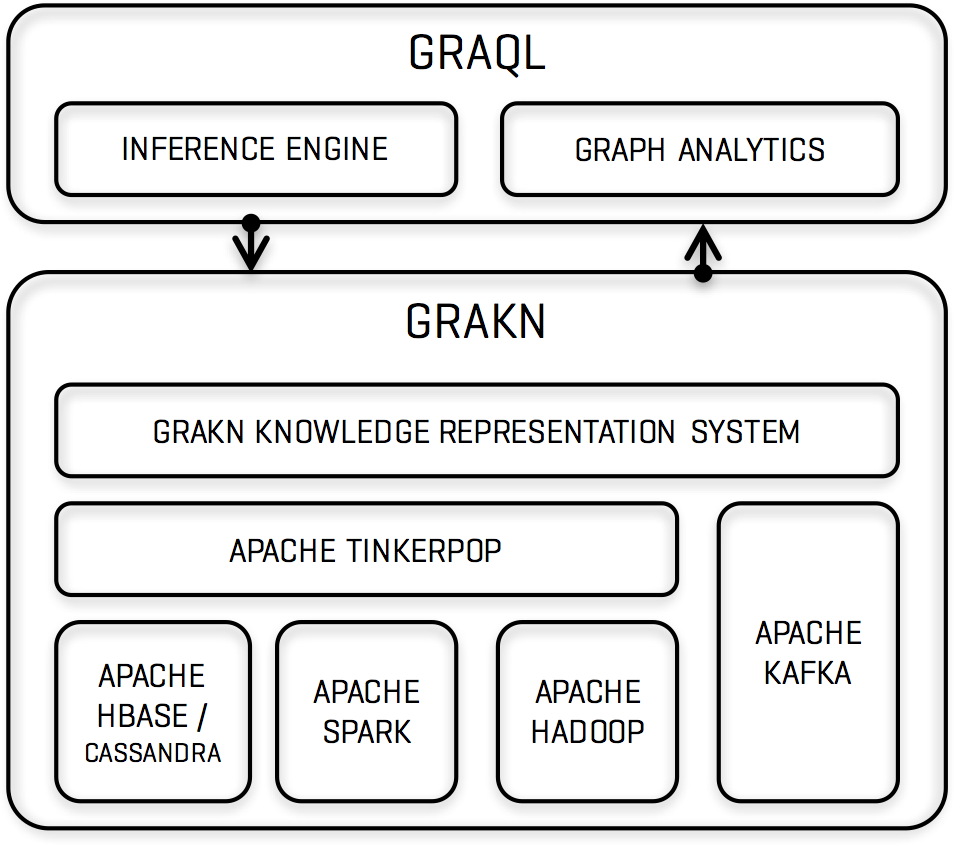
\includegraphics[width=6.8cm]{figures/architecture}
    % \caption{Arquitectura interna de Grakn.
    % Fuente \cite{stichbury}.}
    \caption{Internal architecture of Grakn.
    Source \cite{stichbury}.}
    \label{fig:arch}
\end{figure}

In general, \textit{Grakn} can be seen as a distributed, hyper-relational 
database that uses intuitive\footnote{Refers to the definition of types, 
properties and relationships between existing entities in a given context.} 
ontology\footnote{It should not be seen from the side of philosophy, but as a 
branch of computer science.}  to model complex data, which serves as a 
knowledge base for cognitive systems \cite{dbengines}. On the other side, 
\textit{Graql} is a knowledge-oriented declarative graph query language that 
retrieves knowledge explicitly.
% De manera general, se puede ver a \textit{Grakn} como una base de datos 
% distribuida, hiper-relacional que utiliza una  ontología\footnote{No debe 
% verse desde el lado del la filosofía, sino como una rama de las ciencias de 
% la computación} intuitiva\footnote{se refiere a la definicion de tipos, 
% propiedades y relaciones entre entidades existentes en un determinado 
% contexto} para modelar datos complejos, que sirve como base de conocimiento 
% para los sistemas cognitivos \cite{dbengines}. Por otra parte, \textit{Graql} 
% es un lenguaje de consulta de grafos declarativo orientado al conocimiento 
% (Knowledge-oriented) que recupera conocimiento de manera explícita.

Grakn was designed to be integrated with other technologies that allow it to 
function in a distributed manner. In addition, it is a great complement to 
Natural Language Processing (NLP) and Machine Learning (ML) systems 
\cite{grakn-youtube}. It is also important to note that the data is stored in 
Apache Cassandra, a non-relational database that is distinguished by its speed, 
scale, and simplicity in design.
% Grakn esta diseñado para su integración con otras tecnologías que le permitan 
% funcionar de manera distribuida. Además, es un gran complemento para sistemas 
% de Natural Languaje Processing (NLP) y Machine Learning (ML) 
% \cite{grakn-youtube}. También es importante destacar que los datos son 
% almancenados en Apache Cassandra, una base de datos no relacional que se 
% distingue por su rapidez, escalamiento horizontal y simplicidad en el diseño.

Since Grakn creation in 2016 to present-day, it is use by several international 
companies, such as: Google and Cisco; and by institutions like MIT, OpenCTI, 
and Cares Genetics. Table \ref{fig:grakn-car} summarizes the most important 
features reported by the db-engines \cite{dbengines} site. A more detailed 
explanation can be found on the official Grakn site (\url{https://grakn.ai/}).
% Grakn desde su creación en 2016 hasta la fecha es utilizada por varias 
% trasnacionales, como: Google y Cisco; y por instituciones como MIT, OpenCTI 
% y Cares Genetics. La Tabla \ref{fig:grakn-car} resume las características 
% más importantes que reporta el sitio db-engines \cite{dbengines}. Una 
% explicación con mayor detalle se puede encontrar en el sitio oficial de 
% Grakn (\url{https://grakn.ai/}).

\begin{table}[H]
% \caption{Característica principales de Grakn}
\caption{Grakn main features}
\begin{adjustbox}{width=\columnwidth,center}
\begin{tabular}{|l|l|}
\hline
\textbf{Feature}             & \textbf{Description}                   \\ \hline
% \textbf{Característica}             & \textbf{Descripción}          \\ \hline
Database model                      & Graph DBMS  and relational DBMS \\ \hline
% Modelo de base de datos     & DBMS que usa Grafos y DBMS relacional \\ \hline
Initial release                     & 2016                            \\ \hline
% Lanzamiento inicial                 & 2016                          \\ \hline
Current version                     &  1.7.2, June 2020            \\ \hline
% Versión actual                      & 1.7.2, Junio de 2020          \\ \hline
Origin country                      & United Kingdom               \\ \hline
% País de origen                      & Reino Unido                   \\ \hline
License                             & Open Source                  \\ \hline
% Licencia                            & Open Source                   \\ \hline
Implementing language               & Java                         \\ \hline
% Lenguaje de implementación          & Java                          \\ \hline
Supporting operative systems        & Linux, OS X and Windows      \\ \hline
% Sistemas operativos soportados      & Linux, OS X y Windows         \\ \hline
Triggers                            & no                            \\ \hline
Supporting languages                & 
\begin{tabular}[c]{@{}l@{}}All languages base on JVM:
\\ Groovy,\\ Java,\\ JavaScript (Node.js),\\ Python,\\Scala\end{tabular}\\\hline
% Lenguaje de programación soportados & 
% \begin{tabular}[c]{@{}l@{}}Todos los lenguajes 
% basados en JVM:\\ Groovy,\\ Java,\\ JavaScript (Node.js),\\ Python,\\ 
% Scala\end{tabular} \\ \hline
APIS and other access methods       & 
\begin{tabular}[c]{@{}l@{}}Console (shell),\\ 
gRPC protocol,\\ Workbase (visualisation software)\end{tabular}      \\ \hline
% APIs y otros métodos de acceso      & 
% \begin{tabular}[c]{@{}l@{}}console (shell),\\ 
% gRPC protocol,\\ Workbase (visualisation software)\end{tabular}     \\ \hline
Technical docs                      & https://dev.grakn.ai/­doc         \\ \hline
% Documentación técnica               & https://dev.grakn.ai/­doc  \\ \hline
Usually compare with                & Neo4j, GraphDB y JanusGraph     \\ \hline
% Se compara usualmente con           & Neo4j, GraphDB y JanusGraph   \\ \hline
\end{tabular}
\end{adjustbox}
\label{fig:grakn-car}
\end{table}

\subsection{Grakn installation} % (fold)
% \subsection{Instalación de Grakn} % (fold)

To install Grakn, Java 8 SDK is previously required, if not you can download 
Oracle or OpenJDK implementation. To install Grakn in Linux we can use three 
package managers: \texttt{dnf}, \texttt{yum} (for systems that uses RPM
\footnote{RPM is a recursive acronym which means RPM Package Manager}) 
and \texttt{apt}.
% Para la instalación de Grakn se necesita tener previamente instalado Java 8, 
% en caso de no tenerlo, se puede utilizar la versión proporcionada por Oracle 
% o por OpenJDK. En el caso de Linux, la instalación de Grakn puede hacerse a 
% través de tres gestores de paquetes: \texttt{dnf}, \texttt{yum} (para sistemas 
% que usen gestores RPM\footnote{RPM es un acrónimo recursivo que se desglosa 
% como RPM Package Manager}) y \texttt{apt}.

Besides, Grakn is also available for X OS operative system,  through 
\texttt{brew} package manager. The testing implementations presented in the 
paper were made using CentOS 8.2 and Manjaro Linux 20.0.
% Además, Grakn está disponible también para los sistemas operativos X OS, a 
% través del gestor de paquetes \texttt{brew}. Para este proyecto con el fin de 
% realizar las pruebas de implementación se utilizaron CentOS 8.2 y Manjaro 
% Linux 20.0.

Another important point is that Grakn works similarly to database management 
systems, which means we must start services, create users, workspaces, 
among others. In Grakn the abstract models that encapsulate 
the entities of a particular problem are known as \textit{Keyspace}, where the 
\textit{schemes} that will represent the data of the case study are defined.
% Es importante destacar que Grakn funciona de manera similar a los sistemas 
% manejadores de base de datos, es decir, se deben iniciar servicios, crear 
% usuarios, crear espacios de trabajo, entre otros. En Grakn los modelos 
% abstractos que encapsulan y las entidades de un problema en particular 
% son conocidos como \textit{Keyspace}, donde se definen los \textit{esquemas} 
% que representarán los datos del caso de estudio.

An \textit{scheme} is an inherent part of the knowledge graph that describes 
what data is like and how it can be structured. It can be represented by an 
Entity-Relationship diagram. On the other side, Grakn has various types that 
made up the core system and provide the vocabulary necessary to describe any 
case study. The most important Grakn data types are:
% Un \textit{esquema} es un parte inherente del grafo de conocimiento que 
% describe cómo son los datos y cómo pueden ser estructurados. Dicho esquema 
% se puede representar por medio de un diagrama entidad-relación. En Grakn 
% existen tipos que constituyen el núcleo del esquema y proporcionan el 
% vocabulario necesario para describir cualquier caso de estudio. Entre los 
% principales tipos que maneja Grakn destacan:

\begin{itemize}
    \item \textit{Entities}. They provide the means to classify the objects of 
    a given domain.
    % \item \textit{Entidades}. Proveen los medios para clasificar los 
    % objetos de un dominio.
    \item \textit{Relationships}. They connect the elements, known in Grakn as 
        \textit{things} from a particular domain. They can be objects, 
        relationships y attributes.
    % \item \textit{Relaciones}. Conectan los elementos, conocidos en Grakn 
        % como \textit{things}) de un dominio. Estos pueden ser: objetos, 
        % relaciones y atributos.
    \item \textit{Attributes}. They describe the entities.
    % \item \textit{Atributos}. Son usados para caracterizar las entidades.
\end{itemize}

Likewise, it is important to mention that the query language \textit{Graql} 
has the following characteristics:
% Asimismo, es importante mencionar que el lenguaje de consultas \textit{Graql} 
% presenta las siguientes características, mismas que fueron de utilidad para 
% este trabajo.

\begin{itemize}
    \item \textit{Declarative}. In order to make a query with Graql, it may 
        describe what you want to recover, instead of saying how it should be 
        obtained.
    % \item \textit{Declarativo}. Para hacer una consulta con Graql se tiene 
        % describir lo que se quiere recuperar, en lugar de decir 
        % cómo se debe obtener.
    \item \textit{Intuitive}. Graql was designed to provide a high-level 
        query language interface with clear, readable syntax.
    % \item \textit{Intuitivo}. Graql fue diseñado para proporcionar una 
        % interfaz de lenguaje de consulta de alto nivel con una sintaxis clara 
        % y legible.
\end{itemize}

The operations that can be performed through Graql are data manipulation (DML) 
and data definition (DDL).

\subsection{Semantic relationship schema}
% \subsection{Esquema de las relaciones semánticas}
The semantic characterization created in this work is based on the following 
structure: \texttt{object1--predicate--object2} proposed by \cite{Cewu}, who 
points out that visual relationships capture a wide variety of interactions 
between pairs of objects in images. Therefore, it is recommended to extract the 
possible relationships that may exist, in order to reduce them and work more 
efficiently. Besides, the relations between each pair of objects must 
have a individual predicate, and based on this a classification is made 
to generate a relation. The most common types of predicates are classified 
by an action, space, a preposition, a comparison, or a verb as seen in Figure 
\ref{fig:predaCar}.
% La caracterización semántica creada en este trabajo tiene como base la 
% siguiente estructura: \texttt{objeto1--predicado--objeto2} propuesta por 
% \cite{Cewu}, quienes señalan que las relaciones visuales capturan una amplia 
% variedad de interacciones entre pares de objetos en imágenes. Por lo que, es 
% recomendable hacer una extracción de las posibles relaciones que puedan 
% existir,para así reducirlas y trabajar de una manera más eficiente. Además, 
% se señala que obtener las relaciones entre un par de objetos es necesario que 
% cada uno de estos tenga un predicado de forma individual y con base en esto 
% se realiza una clasificación para generar una relación. Los tipos más comunes 
% de predicados se clasifican por una acción, el espacio, una preposición, 
% una comparación o un verbo como se observa en la Figura \ref{fig:predaCar}.

\begin{figure}[H]
    \centering
    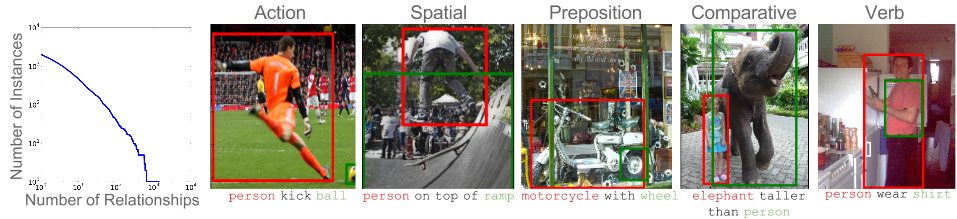
\includegraphics[width=8.8cm]{figures/predica.png}
    \caption{Predicates categorized. Source \cite{Cewu}.}
    \label{fig:predaCar}
\end{figure}

Based on the above, We use the spatial predicates for object characterization, 
since the objects belogns to certain human occupation space, 
such as a room, are static. Whereas, in this case, 
predicates based on verbs (actions) were not useful. In the Figures from 
\ref{fig:abelow} to \ref{fig:topUnder} the relationships used to make the 
knowledge graph are shown.
% Con base en lo anterior, en este trabajo se realizó la caracterización de 
% objetos por medio de predicados espaciales, puesto que los objetos que se 
% encuentran en un determinado espacio de ocupación humana, como una habitación, 
% son estáticos. Mientras que, para este caso, los predicados basados en verbos 
% (acciones) no fueron de utilidad. En las Figuras de \ref{fig:abelow} al 
% \ref{fig:topUnder} se muestran las relaciones que se utilizaron para elaborar 
% el grafo de conocimiento.

\begin{figure}[H]
    \centering
    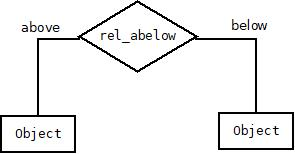
\includegraphics[width=5cm]{figures/abelow.jpg}
    \caption{Relation above-below.}
    \label{fig:abelow}
\end{figure}

\begin{figure}[H]
    \centering
    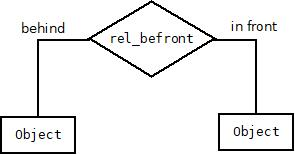
\includegraphics[width=5cm]{figures/befront.jpg}
    \caption{Relation behind-inFront.}
    \label{fig:befront}
\end{figure}

\begin{figure}[H]
    \centering
    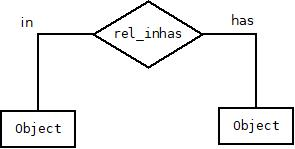
\includegraphics[width=5cm]{figures/inhas.jpg}
    \caption{Relation in-has.}
    \label{fig:inhas}
\end{figure}

\begin{figure}[H]
    \centering
    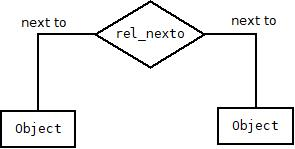
\includegraphics[width=5cm]{figures/nextto.jpg}
    \caption{Relation nextTo.}
    \label{fig:nexto}
\end{figure}

\begin{figure}[H]
    \centering
    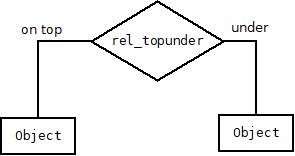
\includegraphics[width=5cm]{figures/topunder.jpg}
    \caption{Relation onTop-under.}
    \label{fig:topUnder}
\end{figure}

The elements recognize as objects have two attributes which are the identifier 
(ID) and the name as shown in Figure \ref{fig:object}. However, as more 
predicates are incorporated, it is possible to add more attributes to the 
object in order to better describe the relationship.
% Los elementos reconocidos como objetos tienen dos atributos los cuales son 
% el identificador (ID) y el nombre como se puede ver en la Figura 
% \ref{fig:object}. Sin embargo, a medida que se vayan incorporando más 
% predicados es posible añadir al objeto más atributos con el fin de describir 
% mejor la relación.


\begin{figure}[H]
    \centering
    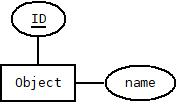
\includegraphics[width=4cm]{figures/object.jpg}
    \caption{Object attributes.}
    % \caption{Atributos de un objeto.}
    \label{fig:object}
\end{figure}

Before implementing the knowledge graph with Grakn, we drafted it, 
to visually identify the relationships that must be created through 
the tool. This conceptual design is seen in Figure \ref{fig:grafo}.
% Antes de implementar el grafo de conocimiento a través de Grakn, se realizó 
% un bosquejo del mismo con la finalidad de identificar de manera visual las 
% relaciones que se deben crear a través de la herramienta. Este diseño 
% conceptual se observa en la Figura \ref{fig:grafo}.

\begin{figure}[H]
    \centering
    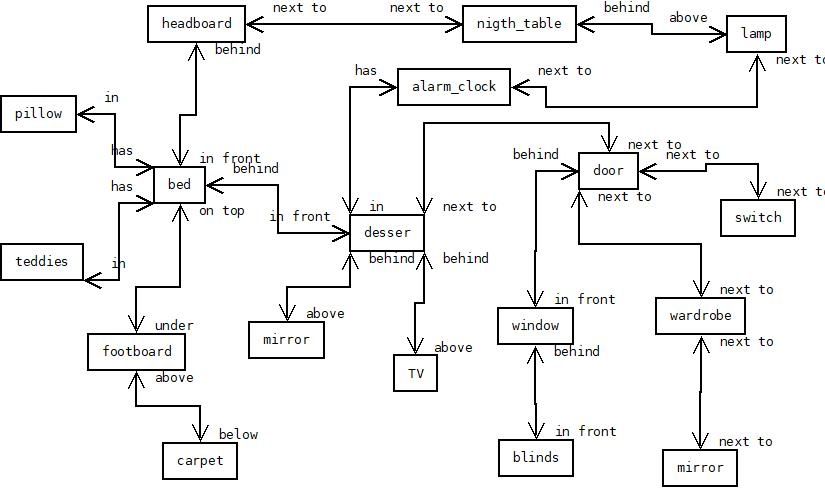
\includegraphics[width=8.8cm]{figures/grafo.jpg}
    \caption{Conceptual design of the knowledge graph.}
    \label{fig:grafo}
\end{figure}

\subsection{Development}
% \subsection{Desarrollo}

The implementation of the knowledge graph in Grakn was based on the previously 
defined relationships scheme, shown in the previous section. Thus, with the 
help of the Graql language, relations of type \texttt{above-below} were defined 
first and then the object, as can be seen in Listing \ref{lst:script1} and 
\ref{lst:script2}, respectively.
% La implementación del grafo de conocimiento en Grakn fue con base en el 
% esquema de las relaciones previamente definidas, mostradas en la sección 
% anterior. Así, con la ayuda del lenguaje Graql se definieron primero las 
% relaciones de tipo \texttt{above-below} y posteriormente el objeto, como 
% se puede ver en Listing \ref{lst:script1} y \ref{lst:script2}, 
% respectivamante.

\lstinputlisting[language=Python, firstline=1, lastline=8,
    caption=Relationship definition using Graql.,
    label={lst:script1}
]{code/schema.gql}
% caption=Definición de las relaciones en 
% Graql,label={lst:script1}]{code/schema.gql}

\lstinputlisting[language=Python, firstline=22, lastline=35,
caption=Object definition using Graql., label={lst:script2}]{code/schema.gql}
% caption=Definición del objeto en Graql,label={lst:script2}]{code/schema.gql}

Later, another script was created to insert the objects, as well as to insert 
the relationships that exist between them. It should be noted that the 
identifier is assigned automatically, so it is not necessary to declare 
it when inserting it. The insertion of the objects is done with the reserved 
word \textit{insert} and the relations with the combination of words 
\textit{insert} and \textit{match}, as seen in Listing \ref{lst:script3} and 
\ref{lst:script4}. A total of seventeen objects were inserted.
% Posteriormente, se creó otro script para insertar los objetos, así como 
% para insertar las relaciones que existen entre éstos. Cabe destacar que el 
% identificador se asigna de manera automática, por lo que, es necesario 
% declararlo a la hora insertarlo. La inserción de los objetos se realiza con 
% la palabra reservada \textit{insert} y las relaciones con la combinación de 
% palabras \textit{insert} y \textit{match}, como se observa en Listing 
% \ref{lst:script3} y \ref{lst:script4}. Se insertaron un total de diecisiete 
% objetos.\\

\lstinputlisting[language=Python, firstline=1, lastline=2,
caption=Object insertion., label={lst:script3}]{code/data.gql}
% caption=Inserción de objetos,label={lst:script3}]{code/data.gql}

\lstinputlisting[language=Python, firstline=62, lastline=65,
caption=Object relationship., label={lst:script4}]{code/data.gql}
% caption=Relación entre los objetos,label={lst:script4}]{code/data.gql}

On the other side, to execute the code it was necessary to create a dedicated 
\textit{keyspace}, which was named \texttt{vision\_relationships}, where the 
schemes and relationships were made. Finally, to check that the objects have 
been inserted correctly, a query was made via console, as shown in Figure 
\ref{fig:correct}. Thus, the created objects were also counted.
% Por otra parte, para ejecutar el código fue necesario crear un 
% \textit{keyspace} dedicado, al cual se nombró \texttt{vision\_relationships}, 
% donde se crean los esquemas y las relaciones mencionadas. Finalmente, para 
% corroborar que los objetos hayan sido insertados correctamente se hizo una 
% consulta vía consola, como se muestra en la Figura \ref{fig:correct}. Así, 
% además se contabilizaron los objetos creados.

\begin{figure}[H]
     \centering
     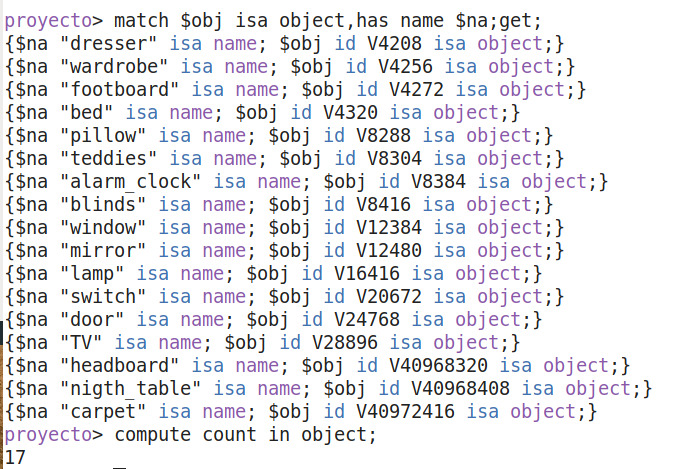
\includegraphics[width=8.8cm]{figures/numObje.jpeg}
     \caption{Query to check that there are no errors.}
    %  \caption{Consulta para corroborar que no existan errores.}
     \label{fig:correct}
\end{figure}
\section{Results}
\label{sec:results}
Figure \ref{fig:grafGra} shows the knowledge graph generated by the query shown in listing \ref{lst:script5}. It is appreciated that the rectangles in purple contain the name of the object and those in fuchsia represent the identifier of the object. Each object can have zero or more relationships to other objects\footnote{Strictly, they only relate to objects that are part of the query.}. However, an object unrelated to others is of no use because it could not be reached since it has no edges, which represent ontological relationships. In addition, implicit or explicit information can be extracted through the edges (green lines).

\lstinputlisting[language=Python, firstline=9, lastline=17,
caption=Query to generate the knowledge graph., label={lst:script5}]{code/queries.gql}

\begin{figure}[H]
    \centering
    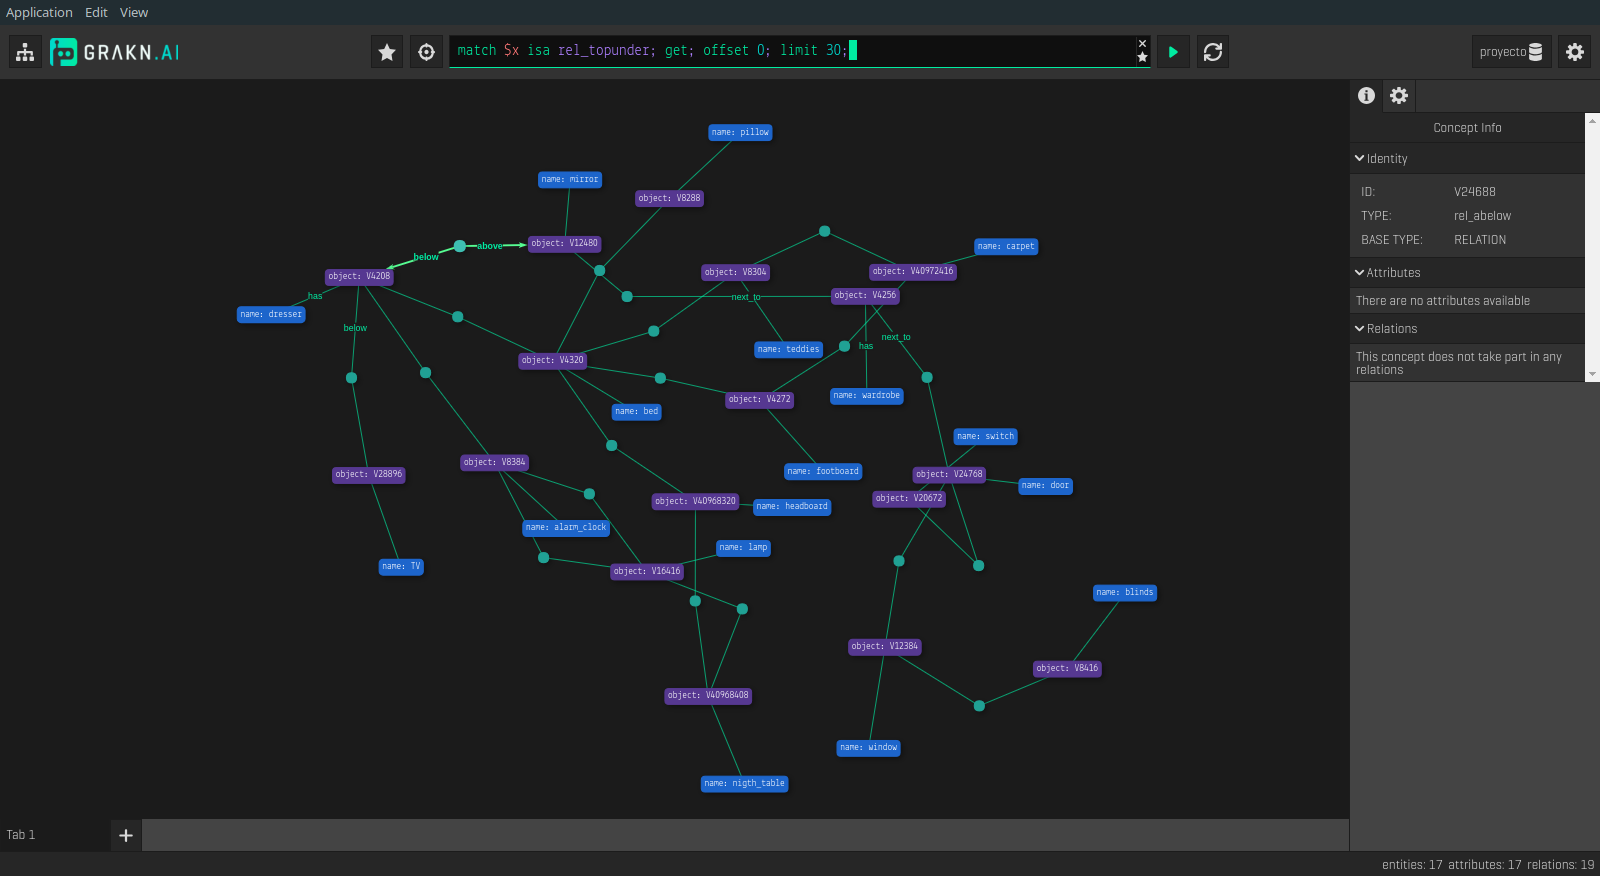
\includegraphics[width=8.8cm]{figures/allrel.png}
    \caption{Knowledge graph in Grakn.}
    % \caption{Grafo en Grakn}
    \label{fig:grafGra}
\end{figure}

The explicit information obtained from the edges explains why the objects were determined to be related. In most cases it is by the nature of the \textit{query} that it is executed. On the other hand, the implicit information is related to the \textit{background} of the relation of objects and is usually used when making inferences, better known as \textit{automatic reasoning}. It is worth mentioning that in this work we only work with explicit relationships.

Figure \ref{fig:ReGra} shows the relationship \textit{rel-topunder} between the bed and footboard which can be expected while finding the object ``footboard'' under the object ``bed'' and the object ``bed'' in top of the ``footboard''. Also, in the same image, the \textit{rel-abelow} relationship between the footboard and carpet can be seen similarly to the previous one.

\begin{figure}[H]
    \centering
    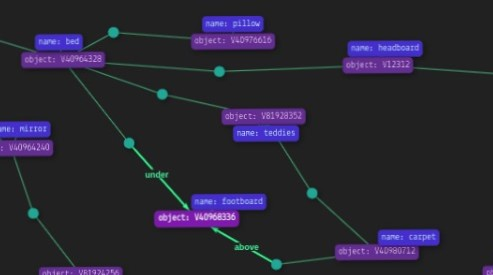
\includegraphics[width=8.4cm]{figures/realcionGrafo.jpeg}
    \caption{Relation bed-footboard, footboard-carpet.}
    % \caption{Relación bed-footboard, footboard-carpet}
    \label{fig:ReGra}
\end{figure}

This work is a contribution to the categorization of the semantic context in computer vision since it establishes the tools and a baseline in spatial relationships to create maps of the environment of places of human occupation, using knowledge graphs, in contrast to the common way it is done.

Normally, to avoid processing an immense quantity of convolutions, which translates into higher execution time, \cite{Galleguillos} suggests creating object context base on object scale or spatial context, by creating big comparison lists (dataset) and contrasting them with image training sets. This is a good approach, however, the list remains static and does not get feedback from the training dataset. Which our model does naturally because that is how knowledge graphs work.
\section{Conclusions}
This work shows that it is possible to create a knowledge graph through semantic relationships, also known as ontological, that exist between objects that are usually found in interior spaces of human occupation, such as a room. In fact, the characterization occurs at the moment of defining the relationship that two objects have to each other, following the convention: \texttt{object1-predicate-object2}.
% Este trabajo muestra que es posible crear un grafo de conocimiento por medio de las relaciones semánticas, conocidas también como ontológicas, que existen entre los objetos que usualmente se encuentran en espacios interiores de ocupación humana, como una habitación. De hecho, la caracterización se da en el momento de definir la relación que tiene dos objetos entre sí, siguiendo la convención sugerida en \cite{Cewu}: \texttt{objeto1--predicado--objeto2}.

Thanks to Grakn it was possible to characterize objects, since through its high-level language it was possible to define the types of highly interconnected relationships between objects, since it provides a scheme that implements the principles of knowledge representation and reasoning.
% Gracias a Grakn fue posible caracterizar los objetos, puesto que por medio de su lenguaje de alto nivel fue posible definir los tipos de relaciones altamente interconectados entre los objetos, ya que proporciona un esquema que implementa los principios de representación del conocimiento y razonamiento.

It is important to highlight that this is an initial work that can be extended depending on the needs and requirements associated with the characterization of objects using knowledge graphs. Its usefulness was shown with the objects present in a room, but the spectrum can also be extended to an entire house, offices, or other closed and open spaces of human occupation.
% Es importante destacar que este es un trabajo inicial que puede extenderse en función de las necesidades y requerimientos asociados a la caracterización de objetos mediante grafos de conocimiento. Se mostró su utilidad con los objetos presentes en una habitación, pero también puede ampliarse el espectro a toda una vivienda, oficinas, u otros espacios cerrados y abiertos de ocupación humana. 

On the other side, since an artificial intelligence project is made up of several parts as needed, for the case in which knowledge graphs are involved, there is a phase of data acquisition and subsequently communicates with other systems that feed it back. This is important because the knowledge generated by the graph can serve as input to other models for object detection, such as convolutional neural networks or using YOLO systems.
% Por otro lado, dado que un proyecto de inteligencia artificial se compone de varias partes según se necesite, para el caso en el que se involucran grafos de conocimiento existe una fase de adquisición de datos y posteriormente se comunica con otros sistemas que lo retroalimentan. Lo anterior resulta importante porque el conocimiento generado por el grafo puede servir como entrada a otros modelos para la detección de objetos, como las redes neuronales convolucionales o utilizando sistemas YOLO.

% NEW
As mentioned, this work creates a semantic relationship of objects of an environment of human occupation given. This information could be useful for CNN models and could be added as an additional layer, called a ``semantic layer''. This layer would work in conjunction with the CNN tagging phase, as shown in Figure \ref{fig:pipeline}.

\begin{figure}[H]
    \centering
    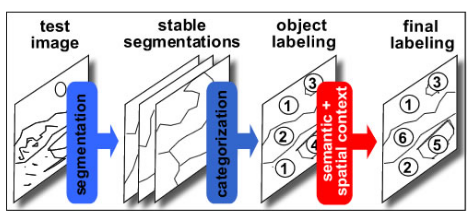
\includegraphics[width=6cm]{figures/pipeline.png}
    \caption{CNN generic pipeline model. Source \cite{Galleguillos2}}
    \label{fig:pipeline}
\end{figure}

% END NEW

Based on the results obtained, and given the usefulness of knowledge graphs in the characterization of objects, future work seeks to create and feed datasets, in JSON, XML or other formats, that contain ontological relationships of existing objects in a given indoor space of human occupation, such as a home, office and other places of rest or work. This will allow an understanding of the environment that surrounds users.
% Con base en los resultados obtenidos, y dada la utilidad de los grafos de conocimiento en la caracterización de objetos, como trabajo futuro se busca crear y alimentar datasets, en formatos JSON, XML u otro, que contengan relaciones ontológicas de objetos existentes en un determinado ambiente cerrado de ocupación humana, como una vivienda, oficina y otros lugares de descanso o trabajo. Esto permitirá comprender el ambiente que rodea a los usuarios. 

On the other side, we will seek to implement an improved version of the knowledge graph, in which new attributes are included, such as the \textit{probability of occurrence} between the relationship of two objects. For this approach, a previous dataset is required, from which we could count the relationships and then translate those data into probabilities.
% Por otro lado, se buscará implementar una versión mejorada del grafo de conocimiento, en el que se incluyan nuevos atributos, como la \textit{probabilidad de ocurrencia} entre la relación de dos objetos. Para este enfoque se requiere de un dataset previo, del cual se puedan hacer conteos de las relaciones y posteriormente traducir esos datos en probabilidades.

% NEW
% b) Otro en las conclusiones, estás son débiles. Necesitas poner alguno relacionado con el objetivo principal que tenías. Se logró o no el cometido de caracterizar objetos a través de la relación semántica y por qué es importante este tipo de análisis.

% IDEAS
% it its important because it allow us to put the right tags in the correct objects, the semantic relationships gives us a lot of contextual information about given objects.

%use our experience
\begin{thebibliography}{00}
\bibitem{Yali}
  Y. Amit and P. Felzenszwalb
  ``Object Detection'',
  \textit{Computer Vision, A Reference Guide}, Springer, 2014
  [E-book] Available: ResearchGate.
  % https://www.researchgate.net/publication/339792032_Object_Detection
  % http://cs.brown.edu/people/pfelzens/papers/detection.pdf
% \bibitem{Ross Girshick}
%   R. Girshick, J. Donahue, T. Darrel and J. Malik,
%   ``Rich feature hierarchies for accurate object detection an semantic
%   segmentation'', \textit{Proceedings of the IEEE conference on computer 
%   vision and pattern recognition}, 2013. [Online serial]. Available: 
%   \texttt{https://arxiv.org/abs/1311.2524} [Accessed Mar. 18, 2020].
\bibitem{Joseph}
  J. Redmon, S. Divvala, R. Girshick and A. Farhadi,
  ``You Only Look Once: Unified, Real-Time Object Detection'',
  \textit{Proceedings of the IEEE conference on computer 
  vision and pattern recognition}, 2015. [Online serial]. Available: 
  \textit{https://arxiv.org/abs/1506.02640} [Accessed Mar. 18, 2020].
\bibitem{Singhal}
  S. Amit, ``Introducing the Knowledge Graph: Things, Not Strings'',
  \textit{Google Official Blog}, 2012. [Online]. Available: 
  \texttt{https://googleblog.blogspot.com} [Accessed: Mar. 20, 2020 ]
\bibitem{Barnard}
  S. van Vessum, ``Grafos de conocimiento: ¿qué son y por qué son
  importantes?'', \textit{ContenKing}, 2019 [Online]. Available:
  \texttt{https://www.contentking.es/blog/grafos-de- \\conocimiento/}
  [Accessed: Mar. 20, 2020]   
\bibitem{Chan}
  C. Niel, ``OK Google, What Is Your Ontology? Or: Exploring Freebase
  Classification to Understand Google’s Knowledge Graph'',
  \textit{arXiv preprint arXiv:1805.03885}, 2019. [Online serial].
  Available: \texttt{https://arxiv.org/abs/1805.03885} [Accessed: Mar. 20, 2020]
\bibitem{Exposito}
  D. Exposito, A. García and A. Martin, ``Grafos'' [Online]
  Available:\texttt{http://decsai.ugr.es/~jfv/ed1/tedi/cdrom/docs/ 
  \\grafos.htm}
  [Accessed: Mar. 21, 2020].
\bibitem{Ehrlinger}
  L. Ehrlinger and W. Wöß, ``Towards a definition of knowledge 
  graphs'', in \textit{Joint Proceedings of the Posters and Demos Track of 12th 
  International Conference on Semantic Systems - SEMANTiCS2016 and 1st 
  International Workshop on Semantic Change \& Evolving Semantics (SuCCESS16)
  At: Leipzig, GermanyVolume: 1695}.
  % \texttt{http://ceur-ws.org/Vol-1695/paper4.pdf}
\bibitem{Toonen}
  E. Toonen, ``What is Google’s Knowledge Graph?'', May, 19 2019. [Online].
  Available: \texttt{https://yoast.com/google-knowledge-graph/}  
  [Accessed: Mar. 21, 2020].
\bibitem{Museo del Prado}
  Museo del Prado, ``El grafo de conocimiento del Museo del Prado'', 
  \textit{Museo del Prado} [Online]. Available: 
  \texttt{https://www.museodelprado.es} [Accessed: May, 26 2020].
  % \texttt{https://www.museodelprado.es/grafo-de-conocimiento/
  % \\el-grafo-de-conocimiento-del-museo-del-prado}
\bibitem{Saorin}
  T. Saorín, ``Grafos de conocimiento y bases de datos en grafo:
  conceptos fundamentales a partir de una obra maestra del Museo del Prado'',
  Anuario ThinkEPI, 2019.
  % Anuario ThinkEPI, v. 13, e13f05, 2019.
\bibitem{Velogig}
  Velogig. ``Knowledge Graphs, graficando el conocimiento'', 
  \textit{Velogig.com}, 2019. [Online]. Available: 
  \texttt{https://velogig.com/knowledge-graphs-graficando-el\\-conocimiento/}.
  [Accessed May, 26 2020].
\bibitem{Fang}
  Y. Fang, K. Kuan, J. Lin, C. Tan and V. Chandrasekhar,
  ``Object Detection. Meets Knowledge Graphs'', 
  \textit{Twenty-Sixth International Joint Conference on Artificial 
  Intelligence}, 2017.
\bibitem{stichbury}
  J. Stichbury. ``Get Started With GRAKN.AI'', \textit{dzone.com}. Mar,10, 2017,
  [Online]. Available: \texttt{https://dzone.com/articles/
  get-started-with-graknai}. [Accessed Jun, 10, 2020].  
\bibitem{dbengines}
  DB-engines, ``Grakn System Properties'', \textit{db-engines.com}.
  [Online]. \texttt{https://dzone.com/articles/get-started-with-graknai}.
  [Accessed Jun, 10 2020].
\bibitem{grakn-youtube}
  Grakn Labs. Online Lecture, Topic: ``Introduction to Knowledge Graphs''.
  \textit{Grakn Labs}, Jun. 10, 2020.
  % \texttt{https://www.youtube.com/watch?v=bCxpNNzbz8M}
\bibitem{Cewu}
  L. Cewu, K. Ranjay, M. Bernstein. L. Fei-Fei.
  ``Visual Relationship Detection with Language Priors'',
  \textit{European Conference on Computer Vision}, 2016
  % Recover on June 11th 2020.
\bibitem{dbpedia}
  DBPedia. ``Ontology'', \textit{dbpedia.org}. [Online]. Available:
  \texttt{https://wiki.dbpedia.org/services-resources/ontology}  
  [Accessed Jun.  22, 2020]  
\bibitem{Galleguillos}
  C. Galleguillos and S. Belongie, ``Context based object categorization: 
  A critical survey'', \textit{Computer Science and Engineering} 
   Computer Vision and Image Understanding, University of California. 2010.
\bibitem{Sadeghi} 
  M. A. Sadeghi and A. Farhadi, ``Recognition using visual phrases'', 
  \textit{CVPR 2011, Providence, RI, 2011, pp. 1745-1752, 
  doi: 10.1109/CVPR.2011.5995711}.
\bibitem{Galleguillos2}
   C. Galleguillos, A. Rabinovich and S. Belongie, ``Object  
   categorization  using  co-occurrence, location and appearance'',
   \textit{ IEEE Computer Society Conference on Computer Vision and Pattern
   Recognition (CVPR 2008)}, Anchorage, Alaska, USA, 2008.
\end{thebibliography}



\end{document}
